\documentclass[12pt, a4paper, oneside]{ctexart}
\usepackage{amsmath, amsthm, amssymb, bm, color, framed, graphicx, hyperref, mathrsfs}

\title{\textbf{4月7日作业}}
\author{韩岳成 524531910029}
\date{\today}
\linespread{1.5}
\definecolor{shadecolor}{RGB}{241, 241, 255}
\newcounter{problemname}
\newenvironment{problem}{\begin{shaded}\stepcounter{problemname}\par\noindent\textbf{题目\arabic{problemname}. }}{\end{shaded}\par}
\newenvironment{solution}{\par\noindent\textbf{解答. }}{\par}
\newenvironment{note}{\par\noindent\textbf{题目\arabic{problemname}的注记. }}{\par}
\everymath{\displaystyle}

\begin{document}

\maketitle

\begin{problem}
【单选】对于一个4输入与门，当输入信号分别为0101和1001，输出信号为（C）
\begin{itemize}
    \item[A ：] 1100 
    \item[B ：] 1101 
    \item[C ：] 0001 
    \item[D ：] 0110 
\end{itemize}
\end{problem}

\begin{problem}
【单选】对于一个4输入异或门，当输入信号分别为0101和1001，输出信号为（A）
\begin{itemize}
    \item[A ：] 1100 
    \item[B ：] 1101 
    \item[C ：] 0001 
    \item[D ：] 0110 
\end{itemize}
\end{problem}

\begin{problem}
【单选】对于半加器和全加器，下列描述正确的是（A）
\begin{itemize}
    \item[A ：] 半加器虽能产生进位输出，但半加器本身并不能处理进位输入 
    \item[B ：] 半加器能产生进位输出，也能处理进位输入 
    \item[C ：] 半加器既不能产生进位输出，也不能处理进位输入 
    \item[D ：] 全加器虽能产生进位输出，但全加器本身并不能处理进位输入 
    \item[E ：] 全加器既不能产生进位输出，也不能处理进位输入 
    \item[F ：] 全加器虽能处理进位输入，但全加器本身并不能产生进位输出
\end{itemize}
\end{problem}

\begin{problem}
【多选】对于“溢出”和“进位”，下列描述正确的是（AB）
\begin{itemize}
    \item[A ：] 有“进位”时，不一定有“溢出” 
    \item[B ：] 有“溢出”时，不一定有“进位” 
    \item[C ：] 有“进位”时，一定有“溢出” 
    \item[D ：] 无“进位”时，一定无“溢出”
\end{itemize}
\end{problem}

\begin{problem}
【单选】为了使十进制表示的算式“8-3”能够在二进制补码加法器上运算，可以表示的形式为（A）
\begin{itemize}
    \item[A ：] 1000+1101 
    \item[B ：] 0011+0011 
    \item[C ：] 1000-1011 
    \item[D ：] 1000-0011 
    \item[E ：] 1000+1011
\end{itemize}
\end{problem}

\begin{problem}
【单选】假设一个基本逻辑门延迟为T，对于8-bit行波进位加法器的关键路径延迟为（C）
\begin{itemize}
    \item[A ：] 15T
    \item[B ：] 16T
    \item[C ：] 17T
    \item[D ：] 18T
\end{itemize}
\end{problem}

\begin{problem}
【单选】超前进行加法器相对于行波进位加法器的优化思路为（A）
\begin{itemize}
    \item[A ：] 提前计算出“进位输出信号” 
    \item[B ：] 简化电路实现的复杂程度 
    \item[C ：] 适用更宽位的加法运算 
    \item[D ：] 节省基本逻辑门之间的连线
\end{itemize}
\end{problem}

\begin{problem}
【单选】关于行波进位加法器和超前进位加法器各自的优缺点描述正确的是（AD）
\begin{itemize}
    \item[A ：] 行波进位加法器门延迟比超前进位加法器更长 
    \item[B ：] 行波进位加法器电路实现更加复杂
    \item[C ：] 超前进位加法器门延迟比行波进位加法器更长 
    \item[D ：] 行波进位加法器电路实现相对简单 
    \item[E ：] 超前进位加法器电路实现更加简单
\end{itemize}
\end{problem}

\begin{problem}
【单选】假设一个基本逻辑门延迟为T，对于8-bit超前进位加法器的关键路径延迟为（C）
\begin{itemize}
    \item[A ：] 2T
    \item[B ：] 3T
    \item[C ：] 4T
    \item[D ：] 5T
\end{itemize}
\end{problem}

\begin{problem}
【单选】对于第一版乘法器（课件第6页），当乘数寄存器最低位为1时，在该次循环过程中，需要将乘数寄存器向哪个方向移动，需要将被乘数寄存器向哪个方向移动？（F）
\begin{itemize}
    \item[A ：] 右，不移动
    \item[B ：] 不移动，左 
    \item[C ：] 不移动，右 
    \item[D ：] 右、右 
    \item[E ：] 左、左 
    \item[F ：] 右、左
\end{itemize}
\end{problem}

\begin{problem}
【多选】对于第一版32-bit乘法器，需要包含以下哪些组成部分？（ABCD）
\begin{itemize}
    \item[A ：] 64位ALU 
    \item[B ：] 32位的乘数寄存器 
    \item[C ：] 64位的被乘数寄存器 
    \item[D ：] 64位的乘积寄存器 
    \item[E ：] 32位ALU 
    \item[F ：] 32位的被乘数寄存器
\end{itemize}
\end{problem}

\begin{problem}
【多选】对于经过流程优化、面积优化后的32-bit乘法器（课件第33页），需要包含以下哪些组成部分？（CEF）
\begin{itemize}
    \item[A ：] 64位ALU 
    \item[B ：] 32位的乘数寄存器 
    \item[C ：] 64位的被乘数寄存器 
    \item[D ：] 64位的乘积寄存器 
    \item[E ：] 32位ALU 
    \item[F ：] 32位的被乘数寄存器
\end{itemize}
\end{problem}

\begin{problem}
【多选】对于第一版32-bit除法器（课件第38页），每次循环都需要判断的条件是哪几个？（AB）
\begin{itemize}
    \item[A ：] 余数寄存器是否小于0 
    \item[B ：] 是否完成了重复了33次循环 
    \item[C ：] 除数寄存器是否小于0 
    \item[D ：] 是否重复了31次循环 
    \item[E ：] 是否重复了32次循环
\end{itemize}
\end{problem}

\begin{problem}
【多选】对于第一版32-bit除法器，需要包含以下哪些组成部分？（ABCD）
\begin{itemize}
    \item[A ：] 64位ALU 
    \item[B ：] 32位的商寄存器 
    \item[C ：] 64位的余数寄存器 
    \item[D ：] 64位的除数寄存器 
    \item[E ：] 32位ALU 
    \item[F ：] 32位的除数寄存器
\end{itemize}
\end{problem}

\begin{problem}
【多选】对于经过流程优化、面积优化后的32-bit除法器（课件第62页），需要包含以下哪些组成部分？（CEF）
\begin{itemize}
    \item[A ：] 64位ALU 
    \item[B ：] 32位的商寄存器 
    \item[C ：] 64位的余数寄存器 
    \item[D ：] 64位的除数寄存器 
    \item[E ：] 32位ALU 
    \item[F ：] 32位的除数寄存器
\end{itemize}
\end{problem}

\begin{problem}
【问答题】考虑基于与非门实现的SR锁存器，请写出下述①-⑥的数值，并说明在什么情况下该SR锁存器的输入是非法的。

% 在此处插入第一张图片
\begin{center}
    % 请将 figure1.png 替换为你本地真实的图片文件名
    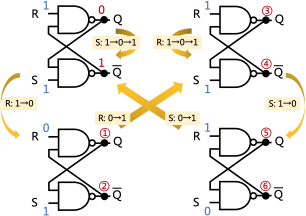
\includegraphics[width=0.6\textwidth]{figure1.png}
\end{center}
\end{problem}

\begin{problem}
【问答题】已知全加器由两个半加器构成，请通过编号说明下述全加器中每个半加器是如何组成的，并写出⑥和⑦分别对应什么输出。

% 在此处插入第二张图片
\begin{center}
    % 请将 figure2.png 替换为你本地真实的图片文件名
    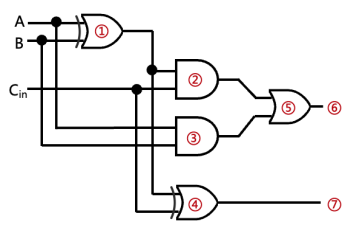
\includegraphics[width=0.6\textwidth]{figure2.png}
\end{center}
\end{problem}

\begin{problem}
【问答题】以4-bit乘法器为例，假设被乘数为0010，乘数为0011，请分别写出第一版乘法器（课件第6页）和经过流程优化、面积优化后的乘法器（课件第33页）在每一轮结束后，乘积寄存器、被乘数寄存器、乘数寄存器（如有）的内容（以二进制表示）。
\end{problem}

\begin{problem}
【问答题】以4-bit除法器为例，假设被除数为0111，除数为0010，请写出第一版除法器（课件第38页）在每一轮结束后，除数寄存器、商寄存器、余数寄存器的内容（以二进制表示）。
\end{problem}

\end{document}